\documentclass{beamer}
\usefonttheme[onlymath]{serif}
\usepackage{amsmath}
\usepackage{amsfonts}
\usepackage[export]{adjustbox}
\usepackage[utf8]{inputenc}
\usepackage{tikz} 
\usepackage{pgffor}
\usetikzlibrary{bayesnet}

% definitions
\def\H{\mathcal{H}}
\def\X{\mathbf{X}}
\def\w{\mathbf{w}}
\def\W{\mathbf{W}}
\def\const{\mathrm{const}}
\def\Var{\mathrm{Var}}
\def\tr{\mathrm{tr}}
\def\T{\top}
\def\U{\mathbf{U}}
\def\S{\mathbf{S}}
\def\V{\mathbf{V}}
\def\N{\mathcal{N}}
\def\E{\mathbb{E}}
\newcommand{\argmin}{\mathop{\mathrm{argmin}}}
\newcommand{\argmax}{\mathop{\mathrm{argmax}}}
\newcommand{\minimize}{\mathop{\mathrm{minimize}}}
\newcommand{\maximize}{\mathop{\mathrm{maximize}}}
\newcommand{\st}{\mathop{\mathrm{subject\,\,to}}}
\newcommand{\mat}[1]{\begin{bmatrix}#1\end{bmatrix}}

%Information to be included in the title page:
\usecolortheme{seahorse}
\title{Bayesian Optimization}
\author{\texorpdfstring{Kangcheng Hou\newline\url{kangchenghou@gmail.com}}{Kangcheng Hou}}

\date{\today}

    
    
\begin{document}
    
\frame{\titlepage}

\begin{frame}{Agenda}
\begin{enumerate}
\item Introduce some attractive examples of Bayesian Optimization.
\item Basic procedure of bayesian optimization without the details of gaussian process or acquisition function.
\item Introduction of gaussian process.
\item Introduction of acquisition function.
\end{enumerate}
\end{frame}


\begin{frame}{Why Bayesian Optimization?}
Bayesian optimization applies when
\begin{itemize}
\item the evaluation of the function that we are trying to optimize is costly. 
\item function is very hard to optimize (hard to compute the gradients)
\item it looks appropriate to model the function using a gaussian process.
\end{itemize}
\end{frame}

\begin{frame}{Attractive Examples}

Some good and successful examples and scenerios where it is great to try bayesopt.

\begin{itemize}
\item hyper-parameter tuning (to evaluate, we need to train the model)
\item Design wet-lab experiments saving time and money. (this is much like the hyper-parameter tuning. Only after that we have done the experiments can we see the final results. Using BayesOpt might help you to find better configuration for the experiments faster with proper prior.
\item usually finds better optima than when tuned by hand
\item honest comparison with other methods for research.
\item the input parameters of the function is formed with discrete and continuous variables.
\end{itemize}
\end{frame}

\begin{frame}
\vspace*{-1pt}
\makebox[\linewidth]{\includegraphics[page=5,width=\paperwidth]{coursera-bml}}
\end{frame}
\begin{frame}
\vspace*{-1pt}
\makebox[\linewidth]{\includegraphics[page=6,width=\paperwidth]{coursera-bml}}
\end{frame}

\begin{frame}[allowframebreaks]{Basic procedure of bayesian optimization}
Take a look as the following function
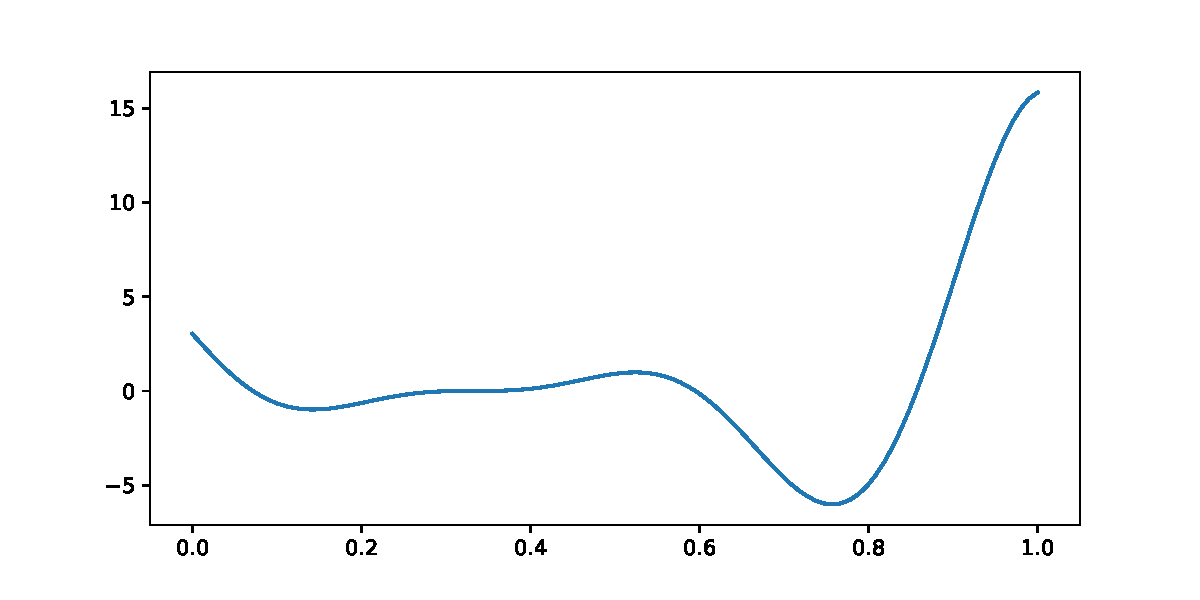
\includegraphics[width=\textwidth]{./img/f}
It has two local minimums and one global minimum. We might think of this stange-shape function as the \texttt{test error - regularization coefficient} graph of some machine learning model(which we don't have access to this function!) 

Think about the process of how we tune the hyper parameter of a machine learning model.
\begin{itemize}
\item We first try some points and evaluate the function value on these points and get some initial function estimates to have a general idea of the function.
\item Then from these estimated points and their function values, we have some sense what the whole function should be like(This is called the surrogate of the original function). We choose to evaluate some point on the original function according to some criterion based on the surrogate to update our posterior to the problem.
\end{itemize}
\end{frame}

\begin{frame}[allowframebreaks]{The procedure}
\foreach \n in {1,...,8}{ \includegraphics[width=\textwidth]{./img/\n} \framebreak}
The red line represents the mean of the distribution of surrogate function while the blue area represents the error area.
\end{frame}

\begin{frame}{Summary of the procedure}
\begin{itemize}
\item Like human, choosing the prior that capture the structure of the problems is very important. (For example, think about why do we assume that the surrogate function is smooth.)
\item the general procedure
\begin{itemize}
    
\item The procedure of bayesian optimization is like we build a surrogate of the black box function that we are trying to optimize. 
\item We perform optimization on the surrogate function distributions based on some criterion to find the good point to evaluate. 
\item We update our belief of the blackbox function i.e. surrogate function with the newly evaluated point.
\end{itemize}
\end{itemize}
\end{frame}

\begin{frame}{Introduction of Gaussian Process}

So how do we represent the surrogate function distribution and update our belief about this?
\begin{itemize}
\item Gaussian Process a.k.a gp provides a great framework to model the distribution of functions. i.e. each sample from gp is a function. or we can think of it as a very high dimension vector.
\item gp provide a systematic way to update our belief i.e. inference for the posterior distribution.
\end{itemize}


\end{frame}

\begin{frame}{Formal representation}
Formally, a gaussian process is determined by two functions, the mean function $m(\cdot)$ and the covariance function $k(\cdot, \cdot)$. A sample from gp is described as follows:
$$f(\cdot) \sim \mathcal{GP}(\mu(\cdot), k(\cdot, \cdot))$$
The sample from GP $f(\cdot)$ satisfies that any $d$ dimensional samples $(f(\mathbf{x}_1), \dots, f(\mathbf{x}_d))$ is from Gaussian distribution $$(f(\mathbf{x}_1), \dots, f(\mathbf{x}_d))^\top \sim \mathcal{N}(\mu(\mathbf{x}_1), \dots, \mu(\mathbf{x}_d)^\top, \mathbf{K}(\mathbf{x}_1, \dots, \mathbf{x}_d))$$
The selection of the mean function $\mu(\cdot)$ and kernel function $k(\cdot, \cdot)$ represents our belief about the sampled function from $\mathcal{GP}$.
\end{frame}

\begin{frame}{Two popular kernels}
Now let's see what kind of belief we make when specifying different $\mu(\cdot)$ and $k(\cdot, \cdot)$.
We will see two kinds of kernels(there are actually tons of other kernels out there!)

Squared exponential

$$k(x, x') = \exp(-\frac{1}{2\tau^2} ||x - x'||^2)$$

Function samples from squared exponential kernel GP is inifinitely differentiable which is not that desired in real life. People turn to use Matérn kernel\footnote{https://en.wikipedia.org/wiki/Mat\%C3\%A9rn\_covariance\_function} for less smooth function samples. Samples from Matérn $\frac{5}{2}$ kernel GP is 2-times differentiable.

$$k(x, x') = \sigma^2 (1 + \frac{\sqrt{5} d}{\rho} + \frac{5d^2 }{3\rho^2}) \exp(-\sqrt{5d}{\rho})$$
The three figures on the left are sampled from RBF kernel, while the right ones are sampled from Matérn kernel GP. 
\end{frame}

\begin{frame}
\begin{columns}[t]
\column{.5\textwidth}
\centering
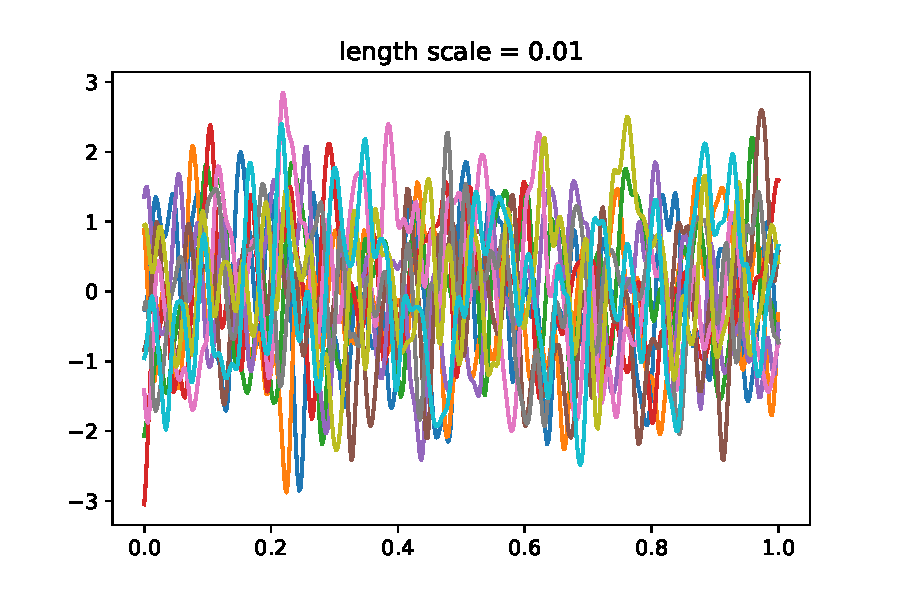
\includegraphics[height=0.3\textheight]{./img/RBF_sample001}
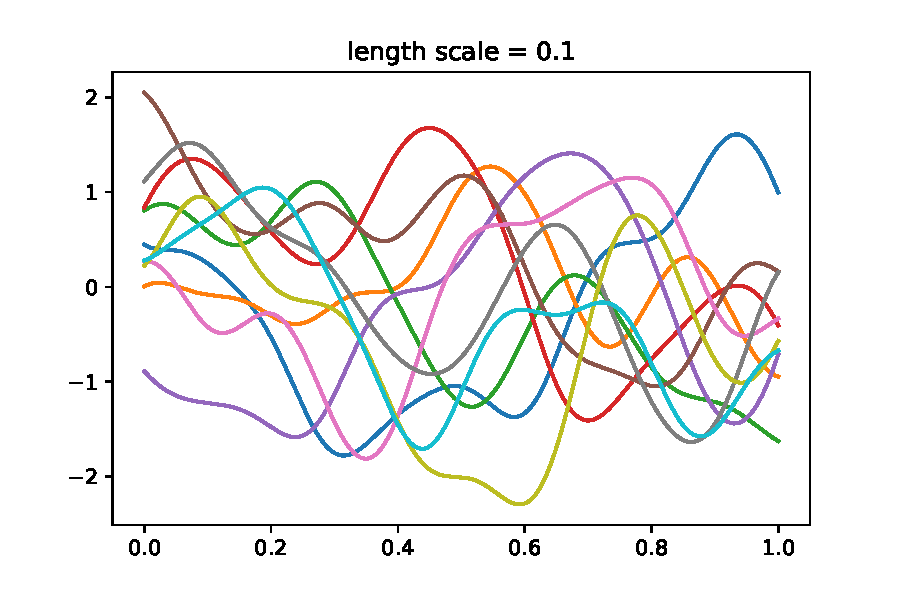
\includegraphics[height=0.3\textheight]{./img/RBF_sample01}
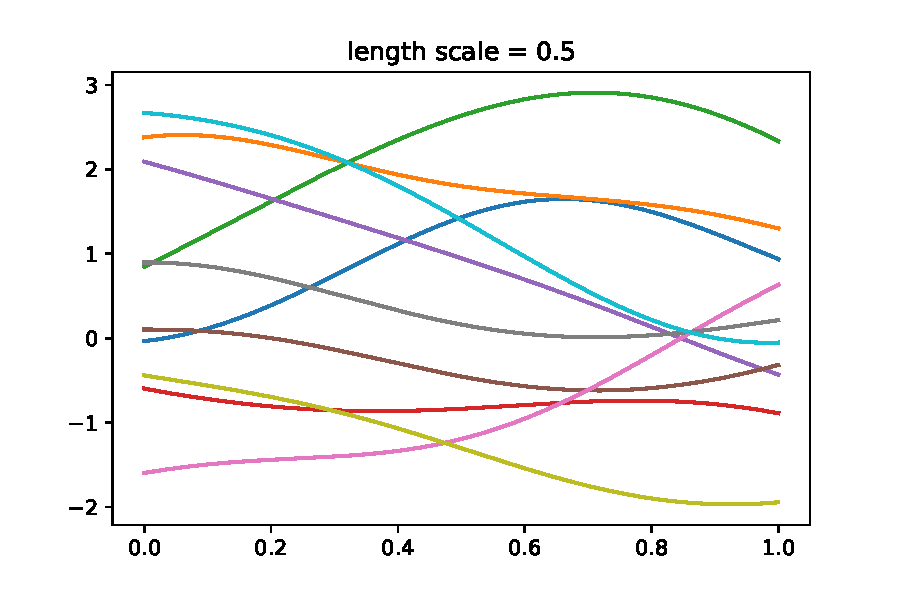
\includegraphics[height=0.3\textheight]{./img/RBF_sample05}
\column{.5\textwidth}
\centering
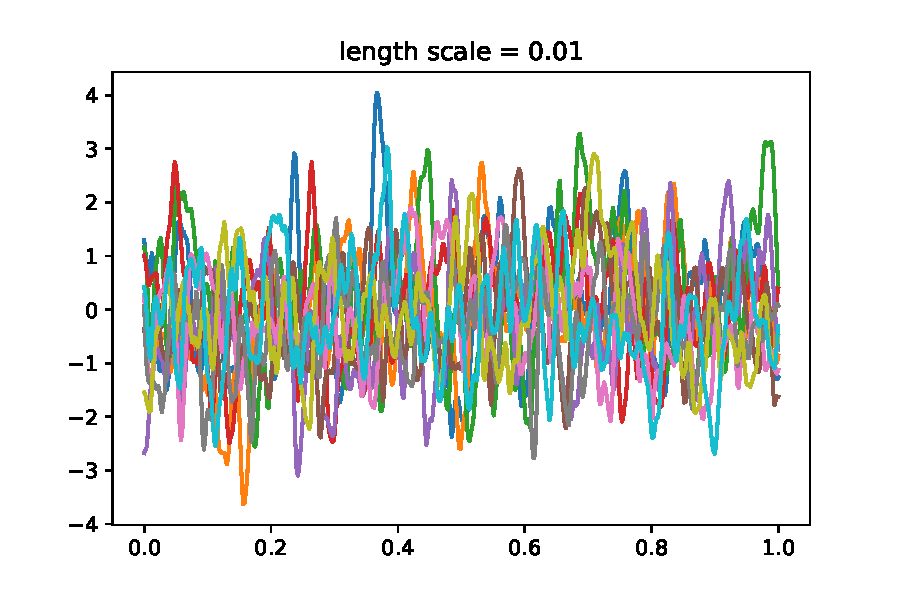
\includegraphics[height=0.3\textheight]{./img/matern_sample001}
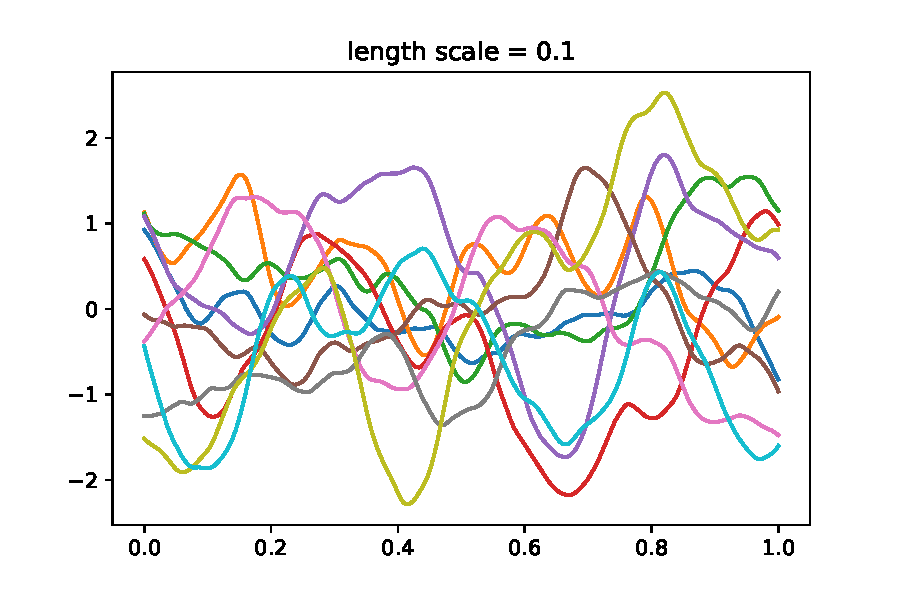
\includegraphics[height=0.3\textheight]{./img/matern_sample01}
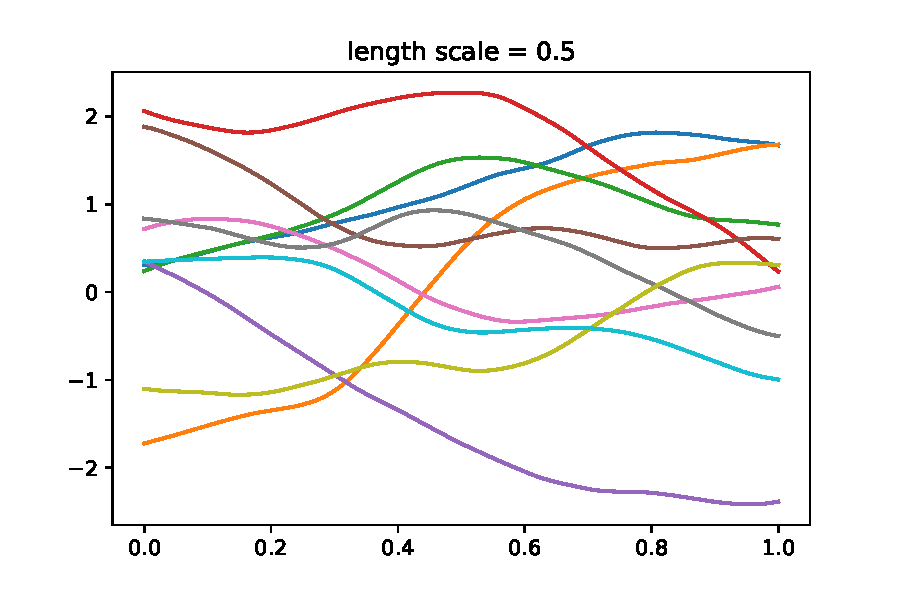
\includegraphics[height=0.3\textheight]{./img/matern_sample05}
\end{columns}
\end{frame}
\begin{frame}{Make our assumptions in mean and covariance function}
Jittering samples may be from financial data while the smoother samples may come from something like weather data.

Choosing the prior depends on what you know about the problems. For example:
\begin{itemize}
\item If we think our data is uptrending. We may assume the mean function has the form $\mu(x) = ax + b, \quad a > 0$.
\item We can choose different kinds of Matérn kernel based on our assumptions about the order of differentiability of the function that we are trying to model.
\end{itemize}
\end{frame}

\begin{frame}{Posterior Inference}
We already know how to sample function from a GP model. Also, we know what are samples like when we use different kernel functions. Once specifying a form of kernel function, we want to know what infer the parameter.
There are basically three kinds of inference methods.(From computationally efficient to inefficient and from approximate to accurate under our prior assumption.) They are 
\begin{itemize}
\item Maximum likelihood estimation
\item Maximum a posterior
\item Full bayesian inference
\end{itemize}
\end{frame}


\begin{frame}[allowframebreaks]{Criterion on what point to evaluate next}
We already know how to construct the surrograte function based on our assumption and update this surrogate after observing new data. Now we introduce how to select the new point to evaluate based on this surrogate function.

The basic principle of point selection is to weight the tradeoff between \textbf{exploration} and \textbf{exploitation}. Noting that our ultimate goal is to find the lowest point of some black box function. We already have some estimated function points. Either we can go deeper for lower function value points or we can explore some points that we are highly uncertain. 


\framebreak 

An creterion that is easy to understand is Lower Confidence Bound acquisition function
$$\alpha(x) = \mu(x) - \kappa \sigma(x)$$
If we take $\kappa=2$ this is just the $\mu(x) - 2\sigma(x)$ line. Think about how it balance the exploration and exploitation. $\mu(x)$ corresponds to exploration while $\sigma(x)$ corresponds to the exploitation.



\begin{figure}
\centering
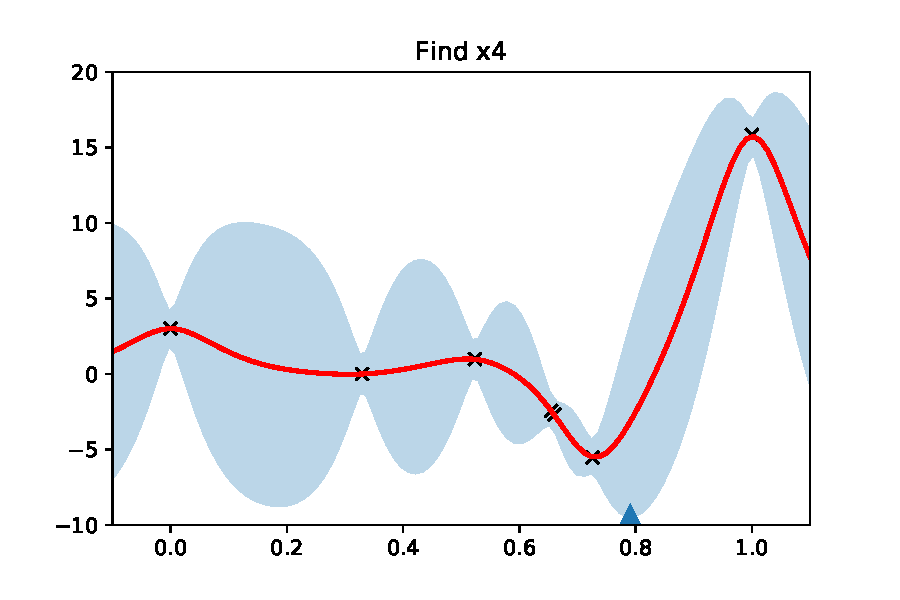
\includegraphics[width=0.8\textwidth]{./img/4}
\end{figure}
\end{frame}

\begin{frame}{Alternaitve acquisition functions}
Alternative choices of acquisition function includes:
\begin{itemize}
\item Expected Improvement
\item Knowledge gradient 
\item Entropy Search
\end{itemize}
\end{frame}

\begin{frame}{Extension of the Bayesian Optimization}
\begin{itemize}
\item Noisy evaluations
\item Parallel Evaluations
\item Constraints
\item Multi-Fidelity and Multi-Information Source Evaluations
\item Random Environmental Conditions and Multi-Task Bayesian Optimization
\end{itemize}
\end{frame}


\begin{frame}{Summary}


\end{frame}
% \begin{frame}{Gaussian Process as function generator}
% Gaussian Process is a distribution over function space, it can be used to represent uncertainty.
% Samples from GP satisfies that any $d$ dimensional samples $(\mathbf{x}_1, \dots, \mathbf{x}_d)$ is from Gaussian distribution $\mathcal{N}(\mu(\mathbf{x}_1), \dots, \mu(\mathbf{x}_d)^\top, \mathbf{K}(\mathbf{x}_1, \dots, \mathbf{x}_d))$ 
% The $\mu$ and $\mathbf{K}$ is chosen to represent our knowledge about the problem.
% So provided some positions to be estimated $(\mathbf{x}_1, \dots, \mathbf{x}_d)$, GP can generate some functions and return the value estimated on those provided input points.
% \end{frame}

% \begin{frame}[allowframebreaks]{Inference in GP}
% First we notice the properties of Gaussian distribuion,
% $$p(\mathbf{f}, \mathbf{g}) = \mathcal{N}(\mat{\mathbf{a}\\\mathbf{b}}, \mat{A & C \\ C^\top &  B})$$
% $$p(\mathbf{f} | \mathbf{g}) = \mathcal{N}(\mathbf{a} + CB^{-1}(\mathbf{y} - \mathbf{b}), A - C B^{-1} C^\top)$$
% In this way, if we know the mean and the covariance of joint distribution of $(\mathbf{f}, \mathbf{g})$ and the observed $\mathbf{g}$. We can then infer the distribution of $\mathbf{f}$. 
% What if we only saw a noisy observation, $\mathbf{y} \sim \mathcal{N}(\mathbf{g}, S)$?

% \framebreak
% $$p(\mathbf{f}, \mathbf{g}, \mathbf{y}) = p(\mathbf{f}, \mathbf{g}) p(\mathbf{y} | \mathbf{g})$$
% is the product of two gaussian pdf, so joint distribution of $(\mathbf{f}, \mathbf{g}, \mathbf{y})$ is still Gaussian distributed.
% Our posterior over $\mathbf{f}$ is still Gaussian:
% $$p(\mathbf{f} | \mathbf{y}) \propto \int d \mathbf{g} p(\mathbf{f}, \mathbf{g}, \mathbf{y})$$
% Thus, we can compute posterior over $\mathbf{f}$ given noisy observation $\mathbf{y}$.

% \framebreak

% Assuming that the data \textbf{are really sampled from } the GP we are using, given
% \begin{align*}
% \text{function }f \sim \mathcal{GP} \\ 
% \mathbf{f} \sim \mathcal{N}(\mu, K) \\
% y_i | f_i \sim \mathcal{N}(f_i, \sigma_n^2)
% \end{align*}
% We can do inference for test points $X_\ast$.
% $$p(\mat{\mathbf{y} \\ \mathbf{f}_\ast}) = \mathcal{N}(\mathbf{0}, \mat{K(X, X) + \sigma_n^2 \mathbb{I} & K(X, X_\ast) \\ K(X_\ast, X) & K(X_\ast, X_\ast)})$$
% Using the previous formula, we can calculate the conditional distritbuion $p(\mathbf{f}_\ast | \mathbf{y})$.
% \end{frame}

% \begin{frame}[allowframebreaks]{Hyper parameters}
% Now if we specify the mean and covariance function, we can then do inference of the test points given the observed value $p(\mathbf{f}_\ast | \mathbf{y})$.
% The natural question to ask is 
% \begin{itemize}
% \item How to determine the mean and covariance function?
% \item What implication we are making if we specify the mean and covariance function?
% \end{itemize}
% Consider an example of Bayesian linear regression,
% $$f(\mathbf{x}_i) = \mathbf{w}^\top \mathbf{x}_i + b, \quad \mathbf{w} \sim \mathcal{N}(0, \sigma_w^2 \mathbb{I}), b \sim \mathcal{N}(0, \sigma_b^2)$$
% \begin{align*}
% \text{cov}(f_i, f_j) & = \langle f_i, f_j \rangle - \langle f_i \rangle \langle f_j \rangle \\ 
% & = \langle \mathbf{w}^\top \mathbf{x}_i + b, \mathbf{w}^\top \mathbf{x}_j + b \rangle \\
% & = \sigma_w^2 \mathbf{x}_i^\top \mathbf{x}_j + \sigma_b^2 = k(\mathbf{x}_i, \mathbf{x}_j)
% \end{align*}
% This means the Bayesian linear regression is equivalent to the $k(\mathbf{x}_i, \mathbf{x}_j) = \sigma_w^2 \mathbf{x}_i^\top \mathbf{x}_j + \sigma_b^2$ kernel. 
% \end{frame}



\end{document}